\begin{EXO}{Variations d'une fonction du second degré}{}
Soit $f$ une fonction définie sur $\R$ par $f(x) = x^2+x-2$.

\begin{tcbenumerate}[3]
\tcbitem \tcbitempoint{1} Calculer $f(1)$

\begin{crep}
$f(1) = 1^2 + 1 - 2 = 0$
\end{crep}

\tcbitem[raster multicolumn=2] \tcbitempoint{2} Déterminer la forme canonique de $f$.

\begin{crep}[extra lines=1]
$f(x) = x^2 + x - 2$, on a  $\alpha = -\dfrac{1}{2 \times 1} = -\dfrac{1}{2}$\\[0.6em]
$\beta = f\left(-\dfrac{1}{2}\right)= \left(-\dfrac{1}{2}\right)^2 + \left(-\dfrac{1}{2}\right) - 2 $\\[0.6em]
$= \dfrac{1}{4} - \dfrac{1}{2} - 2 = -\dfrac{9}{4}$\\[0.6em]
Donc $f(x) = \left(x + \dfrac{1}{2}\right)^2 - \dfrac{9}{4}$
\end{crep}

\tcbitem[raster multicolumn=3] \tcbitempoint{3} Dresser le tableau de variations de $f$.
\setrdcrep{seyes=false,correction color=black,correction font=\normalsize}
\begin{crep}[colframe=white, colback=white]


\begin{center}
\begin{tikzpicture}
\tkzTabInit{$x$/1,$f(x)$/1.2}
{$-\infty$,$-\frac{1}{2}$,$+\infty$}
\tkzTabVar{+/$+\infty$,-/$-\frac{9}{4}$,+/$+\infty$}
\end{tikzpicture}
\end{center}
\end{crep}
\end{tcbenumerate}

\exocorrection

\begin{tcbenumerate}[3]
\tcbitem $f(1) = 1^2 + 1 - 2 = 1 + 1 - 2 = 0$

\tcbitem Pour déterminer la forme canonique de $f(x) = x^2 + x - 2$ :

Coefficient dominant $a = 1 > 0$, coefficient de $x$ : $b = 1$.

$\alpha = -\dfrac{b}{2a} = -\dfrac{1}{2 \times 1} = -\dfrac{1}{2}$

$\beta = f\left(-\dfrac{1}{2}\right) = \left(-\dfrac{1}{2}\right)^2 + \left(-\dfrac{1}{2}\right) - 2$

$\beta = \dfrac{1}{4} - \dfrac{1}{2} - 2 = \dfrac{1}{4} - \dfrac{2}{4} - \dfrac{8}{4} = -\dfrac{9}{4}$

Donc la forme canonique est : $f(x) = \left(x + \dfrac{1}{2}\right)^2 - \dfrac{9}{4}$

\tcbitem Puisque $a = 1 > 0$, la parabole est tournée vers le haut.

La fonction admet un minimum en $x = -\dfrac{1}{2}$ avec $f\left(-\dfrac{1}{2}\right) = -\dfrac{9}{4}$.

La fonction est décroissante sur $\CrochetD-\infty ; -\dfrac{1}{2}\CrochetD$ et croissante sur $\CrochetG-\dfrac{1}{2} ; +\infty\CrochetG$.
\end{tcbenumerate}
\end{EXO}